%! Licence = CC BY-NC-SA 4.0

%! Author = gianfluetsch, mariuszindel
%! Date = 30. Dez 2021
%! Project = cydef_summary


\section{Active Directory}\label{sec:active-directory}

\subsection{Was ist eine AD?}\label{subsec:was-ist-eine-ad}

\subsubsection{Vorteile}
\begin{itemize}
    \item Single-Sign On (Kerberos)
    \item Mit Domänenkennwort an jedem Computer anmelden
    \item Zentrales Management für praktisch alles
\end{itemize}

\subsubsection{Beschreibung}
\begin{itemize}
    \item Active Directory (AD) ist ein Verzeichnisdienst (Datenbank), von Microsoft entwickelt
    \item Wird für die zentralisierte Verwaltung von Computern, Servern, Benutzern, etc. verwendet.
    \item Führt die Authentifizierung und Autorisierung von Benutzern und Computern durch
    \begin{itemize}
        \item Prüft die Anmeldeinformationen der Benutzer und legt ihre Zugriffsrechte fest
        \item Basiert auf LDAP, NTLM, Kerberos (Microsofts Version), DNS und anderen Protokollen
    \end{itemize}
    \item Strukturiert in Objekten
    \begin{itemize}
        \item Ressourcen (z. B. Drucker)
        \item Sicherheitsprinzipien (z. B. Benutzer, Gruppen, Computerkonten)
    \end{itemize}
    \item Organisatorische Einheiten
    \begin{itemize}
        \item Objekte innerhalb einer Domäne können in OUs gruppiert werden
        \item OUs können eine Hierarchie für eine Domäne bilden. Dies vereinfacht die Verwaltung.
    \end{itemize}
    \item Logische Unterteilungen: Forest, tree \& domain
    \item Active Directory speichert
    \begin{itemize}
        \item password hash of every user $\rightarrow$ \textbf{Target for attackers!!!}
        \item computer hash of every computer
    \end{itemize}
\end{itemize}

\subsubsection{Terminologie}
\begin{itemize}
    \item Container
    \begin{itemize}
        \item Übergeordnetes Objekt für bestimmte Arten von AD-Objekten
        \item Forests, Domains, OUs, Sites, subnets
    \end{itemize}
    \item Domain
    \begin{itemize}
        \item Objekte werden immer in einer Domäne gesammelt
        \item Logische Gruppe von Netzwerkobjekten (Computer, Benutzer, Geräte)
        \item Identifiziert durch einen DNS-Namen (Namespace)
    \end{itemize}
    \item Tree
    \begin{itemize}
        \item Sammlung von einer oder mehreren Domänen oder Trees
        \item Verknüpft in einer transitiven Vertrauenshierarchie
    \end{itemize}
    \item Forest
    \begin{itemize}
        \item Einzelne Active Directory-Instanz
        \item Sammlung von Bäumen, die einen gemeinsamen globalen Katalog nutzen
        \item Sicherheitsabgrenzung (Security Boundary)
    \end{itemize}
\end{itemize}

\subsubsection{Security Prinzipien}
Ist eine Entität, die authentifiziert werden kann (z.B.\ Benutzer, Computer, Gruppen)\\
\textbf{SID} (Security Identifier) identifiziert einen Security Principal eindeutig.\\
\begin{center}
    \vspace{-8pt}
    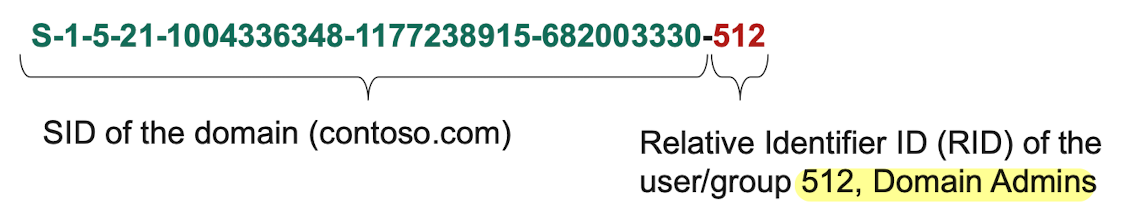
\includegraphics[width=.7\linewidth]{./img/03-active_directory/sid}
    \vspace{-8pt}
\end{center}
SID mit der Relativen Identifier ID (RID) 512 sind Domain Admins und somit für Angreifer von hoher bedeutung!

\subsubsection{ACL: Access Control List}
Eine access control list (ACL) ist eine Liste von access control entries (ACE). ACE spezifiziert die Zugriffsrechte,allowed, denied oder audited. Der security descriptor für ein Objekt kann 2 Typen von ACL beinhalten.
\begin{itemize}
    \item Discretionary Access Control (DACL):\\
    Eine Liste identifiziert die Trustees, denen der Zugriff auf ein sicheres Objekt erlaubt oder verweigert wird
    \item System Access Control (SACL):\\
    Ermöglicht Administratoren die Protokollierung von Zugriffsversuchen auf ein gesichertes Objekt
\end{itemize}

\subsubsection{GPO: Group Policy Objects}
% TODO: Implement

\subsubsection{Administrators}
\begin{itemize}
    \item BUILTIN \textbackslash Administrators\\
    Lokaler Admin-Zugang auf einem Domänencontroller
    \item Domain Admins\\
    Administrativer Zugriff auf alle Ressourcen in der zugehörigen Domäne.
    \item Enterprise Admins\\
    Existiert nur in der Forest Root. Wird implizit zu ,,Domain Admins`` jeder untergeordneten Domain hinzugefügt.
    \item Schema Admins\\
    Kann das Domänen-/Forstschema ändern.
    \item Server Operators\
    Kann Domänenserver verwalten.
    \item Account Operators\\
    Kann jeden Benutzer verwalten, der nicht zu einer ,,privilegierten`` Gruppe gehört.
\end{itemize}

\subsubsection{AD Threats}
Das AD ist ein zentrales Ziel für Angreifer. Ist die AD gefährdet, ist alles gefährdet! Die AD-Infrastruktur kann sehr komplex sein und ist daher schwer zu konfigurieren und zu pflegen. Häufige Fehlkonfigurationen, die von Angreifern missbraucht werden können:
\begin{itemize}
    \item Keine Trennung des privilegierten Zugriffs, z. B. hoch privilegierte Administratoren melden sich interaktiv bei Clients/Servern an
    \item Dienst- (oder Benutzer-) Konten mit schwachen Passwörtern und SPN, noch schlimmer, wenn die Inhaberschaft verloren geht
    \item Schwache Passwörter im Allgemeinen
    \item Gleiches lokales Administrator-Passwort auf allen Computern
    \item Wiederverwendung von Passwörtern im Allgemeinen
    \item Anmeldeinformationen auf Freigaben (z. B. Anmeldeskripte auf SYSVOL), auf die jeder Lese-/Schreibzugriff hat
    \item Fehlen des Prinzips der geringsten Rechte im Allgemeinen (least privilege)
\end{itemize}

\subsection{Active Directory Information Gathering}\label{subsec:active-directory-information-gathering}

\subsubsection{ADUC: Active Directory Users \& Computers}
Wird normalerweise zur konfiguration benutzt.

\subsubsection{AD Explorer}
when you don’t have ADUC, use Sysinternals tools

\subsubsection{Net Tools}
Im Terminal

\subsubsection{WMI: Windows Management Instrumentation}
WMI (terminal tool) wird unterschätzt und kann viele Dinge tun:
\begin{itemize}
    \item Laufende Prozesse auflisten
    \item Installierte Antivirenprogramme auflisten
    \item Installierte Updates auflisten
    \item Benutzer, Computer und Gruppen in der Domäne auflisten
    \item Dateien und Registry lesen
    \item Prozess erstellen (lokal oder remote)
    \item RDP aktivieren (lokal oder remote)
\end{itemize}

\subsubsection{PingCastle}
Ping Castle ist ein Tool zur schnellen Bewertung des Sicherheitsniveaus von Active Directory mit einer Methodik, die auf einer Risikobewertung basiert. Hauptfeatures:
\begin{itemize}
    \item Health-check der Domäne
    \item Kartographie der Domänen-Trusts
    \item Scanner für verschiedene Einstellungen (LAPS, Lokale Admins, Shares, SMB, Spooler)
\end{itemize}

\subsection{AADDS: Azure Active Directory Domain Services}\label{subsec:aadds}
\begin{itemize}
    \item Cloud-Lösung von Microsoft
    \item Gleiche Idee wie bei Active Directory vor Ort
    \item Zentral verwaltete "Domäne" für Enterprise Admins
    \item GPO nicht zu 100\% in Azure verfügbar
    \item Richtlinie jetzt im Endpoint Manger Interface von Azure
    \item Bedingte Zugriffskontrolle (MDM, Mobile Device Management)
    \item verwendet OpenID Connect und SAML 2.0
    \item SAML 2.0 wird in der Regel für Identitätsanbieter wie Active Directory Federation Services verwendet
\end{itemize}

\subsection{GPO: Group Policy Objects}\label{subsec:gpo:-group-policy-objects}

\subsubsection{SYSVOL}
\begin{itemize}
    \item Das System-Volume (SYSVOL) ist ein spezielles Verzeichnis auf jedem DC
    \item Besteht aus mehreren Ordnern, von denen einer gemeinsam genutzt wird und als SYSVOL-Freigabe bezeichnet wird.
    \item Der Standardspeicherort ist \%SYSTEMROOT\%\textbackslash SYSVOL\textbackslash sysvol
    \item Kann während DC-Promotion-Prozesses oder später geändert werden.
    \item SYSVOL setzt sich aus Ordnern zusammen:
    \begin{itemize}
        \item Gruppenrichtlinienvorlagen (GPTs), die über die SYSVOL-Replikation repliziert werden.
        \item Der Gruppenrichtlinien Container (GPC) wird über die Active Directory-Replikation repliziert.
        \item Skripte, wie z. B. Startskripte, auf die in einem GPO verwiesen wird.
    \end{itemize}
\end{itemize}

\subsubsection{GPO}
\begin{itemize}
    \item Ein Gruppenrichtlinienobjekt (GPO) ist eine virtuelle Sammlung von Richtlinien Einstellungen.
    \item Ein GPO hat einen eindeutigen Namen, z. B. eine GUID.
    \item Gruppenrichtlinieneinstellungen sind in einem GPO enthalten. Ein GPO kann Richtlinieneinstellungen im Dateisystem und im Active Directory darstellen.
    \item Die GPO-Einstellungen werden von den Clients ausgewertet.
    \item Um eine Gruppenrichtlinie zu erstellen, kann ein Administrator den Group Policy Object Editor verwenden
\end{itemize}

\subsubsection{Folder Policy}
\begin{itemize}
    \item Erstellt ein Ordner auf jedem Computer in der Domain
\end{itemize}

\subsubsection{File Policy}
\begin{itemize}
    \item Erstellt ein File auf jedem Computer in der Domain
    \item Source (z.B. SYSVOL) und Destination (z.B. C-Laufwerk) wird angegeben
\end{itemize}

\subsubsection{Applying Policy}
\textbf{Auf Server direkt}
\begin{itemize}
    \item Auf dem server als Admin \texttt{\small gpupdate/force} in cmd.exe ausführen
\end{itemize}

\textbf{Auf DC für alle}
%TODO: Check if compiled correctly
\begin{itemize}
    \item Auf Domain Controller PowerShell öffnen als Admin
    \item \texttt{\small \$computers = Get-ADComputer -Filter *}
    \item \texttt{\small \$computers | ForEach-Object -Process {Invoke-GPUpdate -Computer \$\_.name -RandomDelayInMinutes 0 -Force}}
\end{itemize}

\subsubsection{Execute Script via GPO}
\begin{itemize}
    \item GPO Editor
    \item Policies $\rightarrow$ Preferences $\rightarrow$ Control Panel Settings
    \item Schedule Task
    \item Select Location of script
\end{itemize}

%
% TODO: Move
%\subsection{Kerberos}
%\begin{minipage}{0.45\linewidth}
%    \begin{enumerate}
%        \item Client $\rightarrow$ TGS (Ticket Granting Server = DC): \textit{Anfrage}
%        \item TGS $\rightarrow$ Client: \textit{TGT (Ticket Granting Ticket)}
%        \item Client $\rightarrow$ Fileserver (FS): \textit{TGT}
%        \item FS $\rightarrow$ Client: \textit{schön und gut, will aber spezifisches Ticket}
%        \item Client $\rightarrow$ TGS: \textit{Anfrage spezifisches Ticket für FS}
%        \item TGS $\rightarrow$ Client: \textit{(spezifisches) Ticket für FS}
%        \item Client $\rightarrow$ FS: \textit{(spezifisches) Ticket für FS}
%        \item FS $\rightarrow$ Client: \textit{alles ok}
%    \end{enumerate}
%\end{minipage}
%\begin{minipage}{0.5\linewidth}
%    \begin{center}
%        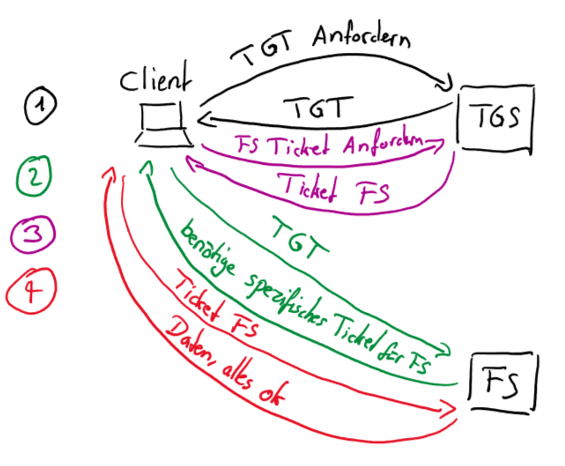
\includegraphics[width=0.9\linewidth]{kerberos}
%        \vspace{-8pt}
%    \end{center}
%\end{minipage}
%
%

